\documentclass{article}
\usepackage[utf8]{inputenc}
\usepackage{amsmath}
\usepackage{amssymb}
\usepackage{graphicx}
\usepackage{hyperref}
\usepackage{caption}
\usepackage[french]{babel}
\usepackage{subcaption}
\usepackage{float} % For [H] placement specifier
\usepackage[T1]{fontenc}
\usepackage{lipsum} % For dummy text

\title{Groupe de Lecture sur l'intelligence artificielle\\GAN}
\author{Julien Chemillier}
\date{2025}

\begin{document}

\maketitle

\section{Introduction}

Ce papier est un résumé du groupe de Lecture sur l'Intelligence Artificielle que j'ai eu la chance d'effectuer
au deuxième semestre de ma L3 à l'Ecole Normale Supérieure de Lyon sur l'année scolaire 2024/2025. \\
Il établit un compte rendu du travail que j'ai fourni sur les \textbf{\href{https://arxiv.org/pdf/1406.2661}{Generative Adversarial Networks}} issus
du papier de recherche de 2014. Ce compte
rendu se veut le plus accessible possible à partir de seules connaissances sur les réseaux de neurones. Il a pour
but de résumer mon expérience et ne pourra donc en aucun cas être un résumé exhaustif du papier de recherche.

\section{Explication du fonctionnement d'un GAN}
\subsection{Construction de l'intuition}
Le GAN est une classe d'algorithme d'apprentissage dont l'objectif est de générer des données similaires à celles
du jeu de données d'entraînement. Pour ce faire, il utilise un fonctionnement relativement novateur. En effet, il
s'agit non pas d'un mais de deux modèles qui s'entraînent simultanément, l'un nommé \textbf{générateur} et l'autre
nommé \textbf{discriminateur}. Ils s'entraînent non seulement simultanément mais surtout conjointement puisqu'ils
essaient tous les deux d'apprendre des erreurs de l'autre. Cette opposition est telle que l'on peut voir le GAN comme
un jeu à deux joueurs: le Générateur et le Discriminateur. \\

L'objectif du discriminateur est de discriminer les images venant du jeu d'entraînement et les autres. \\
L'objectif du générateur est de produire des données ressemblantes à celles du jeu de données d'entraînement pour
essayer de tromper le discriminateur. \\

La seconde particularité de cette approche est que le générateur se met à jour dans le seul but de tromper un peu
plus le discriminateur, c'est-à-dire qu'il ne voit jamais les données du jeu d'entraînement mais seulement la
manière de modifier son comportement pour faire baisser les performances du discriminateur. Ce qui permet
indirectement de réduire l'overfitting même si, on le verra, il est toujours possible d'en avoir.
On dit que le GAN converge lorsque le générateur devient si puissant que le discriminateur n'arrive plus à faire
la différence entre les données du jeu d'entraînement et celles produites par le générateur. On a dans ce cas, un
générateur normalement suffisant pour générer les données que l'on souhaite. \\

Une analogie effectuée dans le papier de recherche originel est celle du faussaire et d'un expert d'authenticité
dans la gestion d'œuvres d'art. L'expert va établir certains critères à partir des œuvres qu'il sait authentiques
pour juger de l'authenticité d'œuvres inconnues. Le faussaire va essayer de générer de nouvelles œuvres d'art en
s'améliorant justement sur les critères que l'expert utilise.
Le GAN est donc une approche algorithmique innovante qui peut s'appliquer à générer des données dans divers domaines.

\subsection{Un peu plus de technicité}
Notons $G$ ($\mathcal{A} \longrightarrow \mathcal{B}$) le générateur et $D$ ($\mathcal{B} \longrightarrow \mathbb{R}$)
le discriminateur et $p_e$ ($\mathcal{B}$) la distribution suivie par le jeu de données d'entraînement.
Pour obtenir une génération de données aléatoires de la part du générateur, il nous faut une part d'aléatoire. C'est
pour cela que l'on va tirer un paramètre $x$ selon une certaine distribution $p_x$. Et cette donnée va servir de au
générateur pour produire des données différents, ainsi $G(x)$ suit $p_g$ qui dépend de $p_x$ et de $G$.
$D(x)$ est la fonction du discriminateur qui estime sa confiance en probabilité que $x$ soit une donnée du jeu
d'entraînement plutôt que de $p_g$.
Soit $V$ la fonction de valeur du jeu qui mesure à quel point $D$ gagne par rapport à $G$. Donc $D$ veut maximiser
$V(G, D)$ alors que $G$ veut le minimiser.
Autrement dit, on cherche:
$$ \min_G \max_D V(G, D) = \mathbb{E}_{e \sim p_e}[\log(D(e))] - \mathbb{E}_{x \sim p_x} [\log(D(G(x)))] $$
Maintenant que l'on sait ce que l'on souhaite atteindre, il nous reste plus qu'à savoir comment faire évoluer G et D pour
atteindre cet équilibre.
Pour ce faire, il suffit d'effectuer une \textbf{descente de gradient} sur la fonction du jeu $V(G, D)$.
En notant $\theta_G$ les paramètres du générateur, $\theta_D$ ceux du discriminateur et $\eta$ le pas
d'apprentissage, il suffit d'appliquer les lignes suivantes:
\begin{itemize}
    \item $ \theta_G = \theta_G - \eta \times \frac{\partial V}{\partial\theta_G} $
    \item $ \theta_D = \theta_D + \eta \times \frac{\partial V}{\partial\theta_D} $
\end{itemize}

\section{Travail effectué}

\subsection{Génération d'images de MNIST}
Pour découvrir l'univers des GAN, rien de tel qu'essayer de générer des images à l'aide de modules préexistants.
Pour cela on va s'appuyer sur le module \textbf{Torch} qui va permettre de générer des réseaux de neurones adaptés
à la situation. MNIST est ici utilisée comme base de données en raison de sa difficulté relativement faible tout en
ayant une grande quantité de données disponible.
On affiche ensuite régulièrement des données construites par le générateur avec un même bruit au fur et à mesure
de l'entraînement pour visualiser cette progression. De cette manière on voit l'évolution du générateur pour un
même bruit:

\begin{figure}[H]
    \centering
    \begin{tabular}{ccccc}
        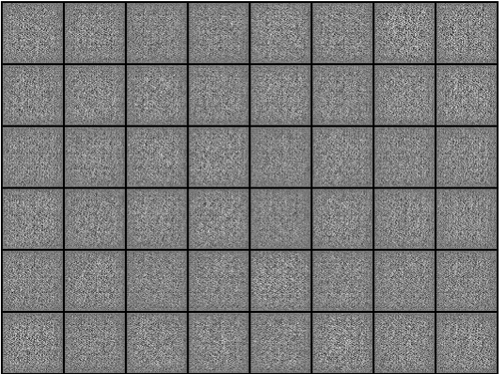
\includegraphics[width=0.18\textwidth]{/images_GAN_MNIST/epoch_1.png} &
        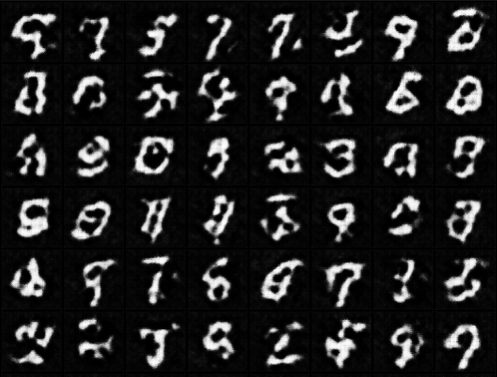
\includegraphics[width=0.18\textwidth]{/images_GAN_MNIST/epoch_2.png} &
        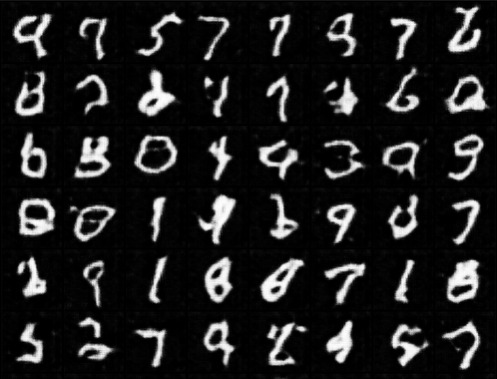
\includegraphics[width=0.18\textwidth]{/images_GAN_MNIST/epoch_3.png} &
        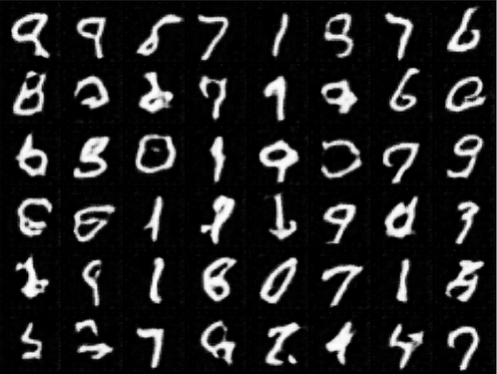
\includegraphics[width=0.18\textwidth]{/images_GAN_MNIST/epoch_4.png} &
        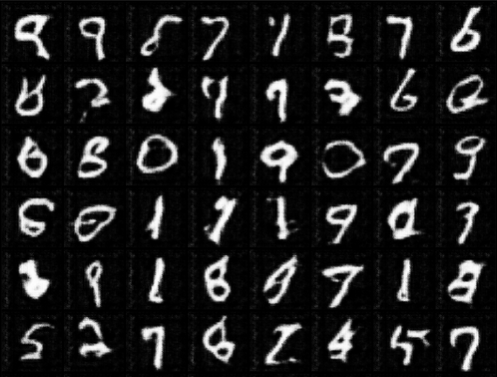
\includegraphics[width=0.18\textwidth]{/images_GAN_MNIST/epoch_5.png} \\
        Epoque 1 & Epoque 2 & Epoque 3 & Epoque 4 & Epoque 5 \\
        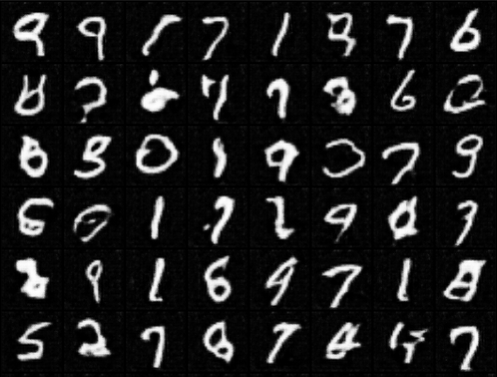
\includegraphics[width=0.18\textwidth]{/images_GAN_MNIST/epoch_6.png} &
        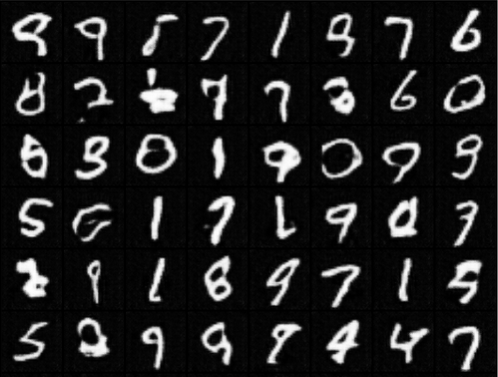
\includegraphics[width=0.18\textwidth]{/images_GAN_MNIST/epoch_7.png} &
        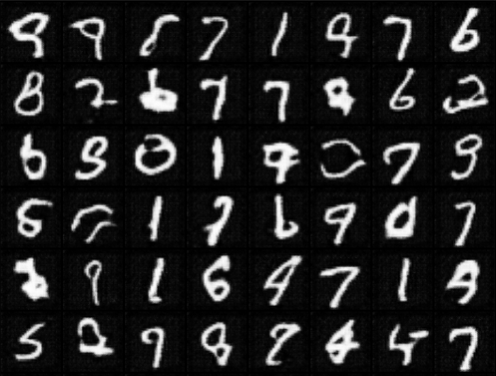
\includegraphics[width=0.18\textwidth]{/images_GAN_MNIST/epoch_8.png} &
        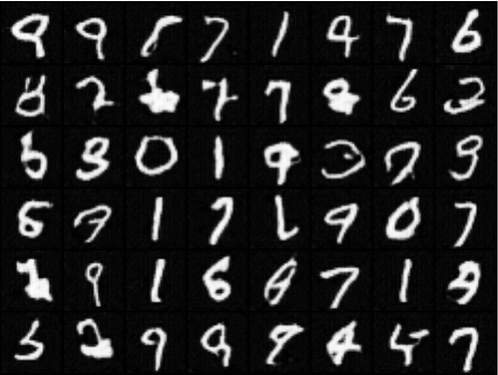
\includegraphics[width=0.18\textwidth]{/images_GAN_MNIST/epoch_9.png} &
        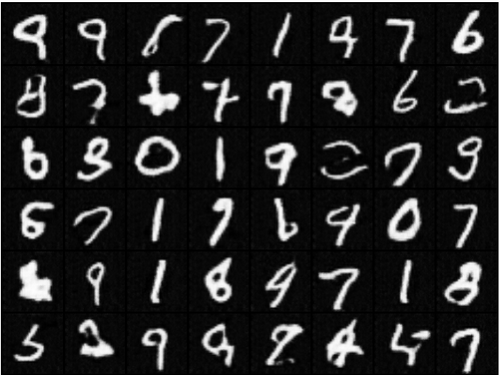
\includegraphics[width=0.18\textwidth]{/images_GAN_MNIST/epoch_10.png} \\
        Epoque 6 & Epoque 7 & Epoque 8 & Epoque 9 & Epoque 10 \\
    \end{tabular}
    \caption{Évolution du générateur sur le jeu de données MNIST}
\end{figure}
Le code permettant de générer de telles images se trouve \href{/gan_on_mnist.py}{ici}.
Google Colab a été utilisé pour générer ces images à l'aide d'un GPU T4 mais le programme fonctionne également sur
un simple CPU (le temps d'attente sera simplement plus long).

\subsection{Génération d'images de visages}
Au vu des performances sur MNIST, je me suis mis en quête de trouver un jeu de données plus corsé. C'est pourquoi
je me suis attaqué à Olivetti faces, un jeu de données de visages de 40 personnes différentes avec 10 images par
personne, soit 400 images au total. La difficulté ici pour le GAN est donc de comprendre l'anatomie du visage malgré
le faible nombre d'images.
Et il s'avère que l'architecture utilisée pour MNIST ci-dessus fonctionne tout aussi bien sur les visages. La seule
subtilité à laquelle il fallait s'attendre en raison du faible nombre de données est la quantité d'époques à
faire avant d'obtenir un résultat convenable.
De la même manière qu'au-dessus, on utilise un même bruit pour observer l'évolution des performances du générateur:
\begin{figure}[H]
    \centering
    \begin{tabular}{ccccc}
        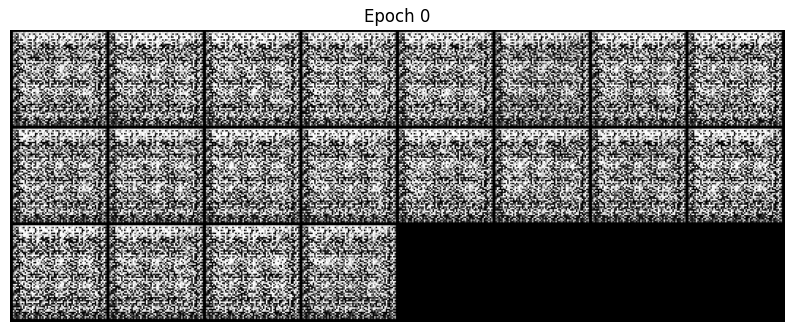
\includegraphics[width=0.45\textwidth]{/images_GAN_Olivetti_faces/epoch_0.png} &
        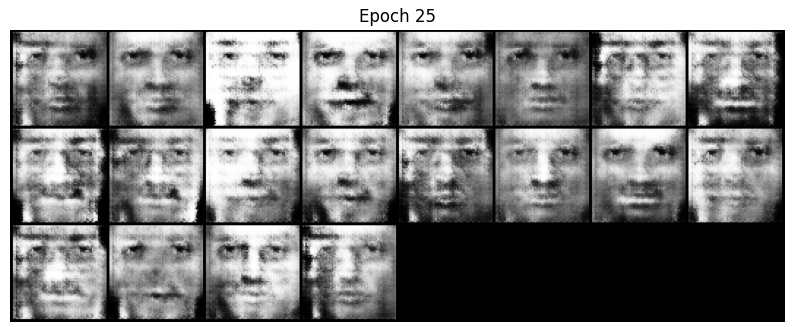
\includegraphics[width=0.45\textwidth]{/images_GAN_Olivetti_faces/epoch_25.png} \\
        Epoque 0 & Epoque 25 \\
        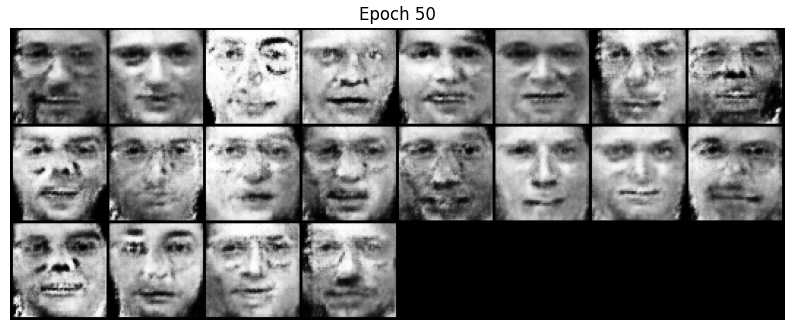
\includegraphics[width=0.45\textwidth]{/images_GAN_Olivetti_faces/epoch_50.png} &
        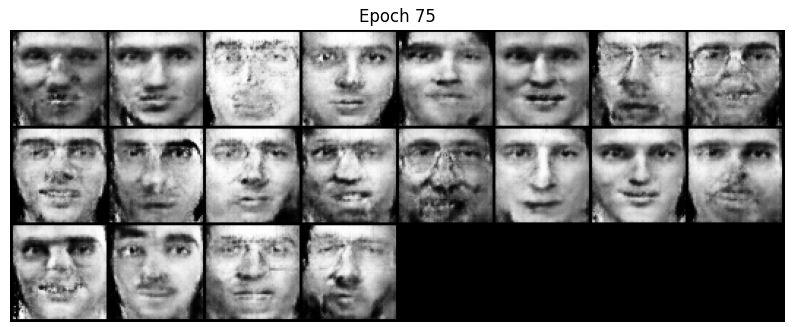
\includegraphics[width=0.45\textwidth]{/images_GAN_Olivetti_faces/epoch_75.png} \\
        Epoque 50 & Epoque 75 \\
        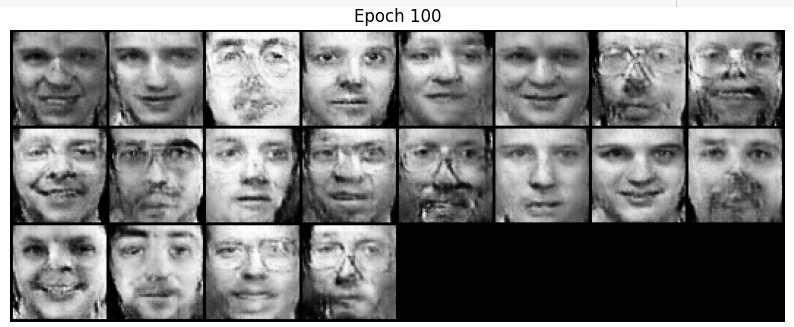
\includegraphics[width=0.45\textwidth]{/images_GAN_Olivetti_faces/epoch_100.png} &
        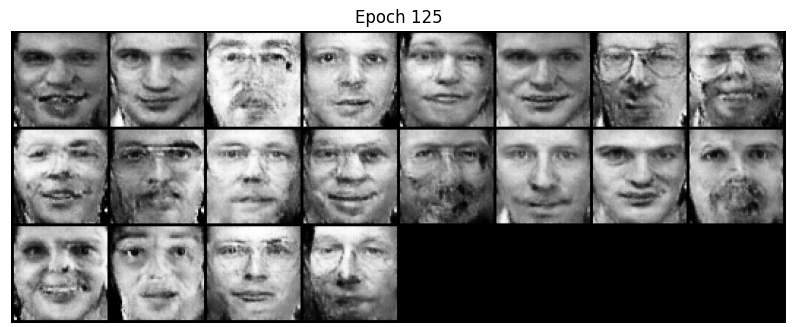
\includegraphics[width=0.45\textwidth]{/images_GAN_Olivetti_faces/epoch_125.png} \\
        Epoque 100 & Epoque 125 \\
        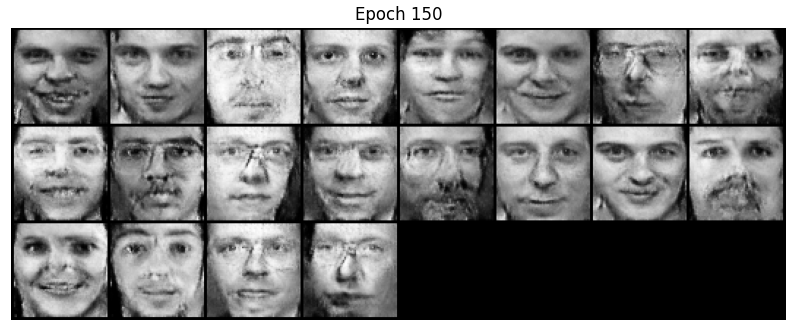
\includegraphics[width=0.45\textwidth]{/images_GAN_Olivetti_faces/epoch_150.png} &
        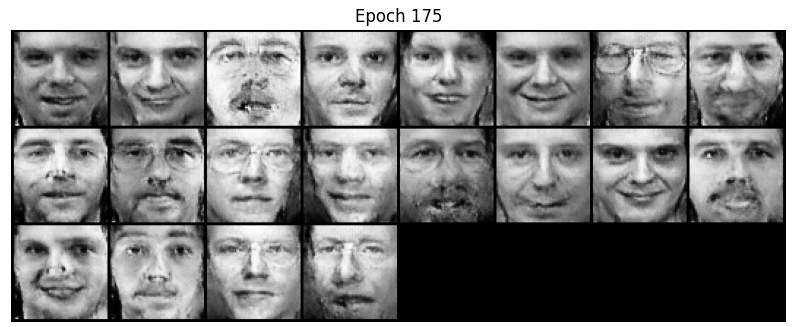
\includegraphics[width=0.45\textwidth]{/images_GAN_Olivetti_faces/epoch_175.png} \\
        Epoque 150 & Epoque 175 \\
        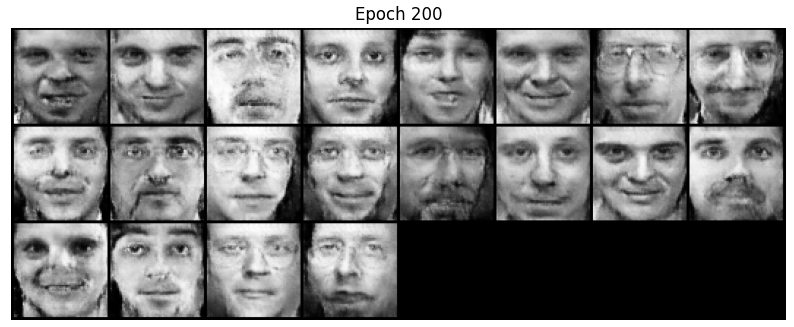
\includegraphics[width=0.45\textwidth]{/images_GAN_Olivetti_faces/epoch_200.png} &
        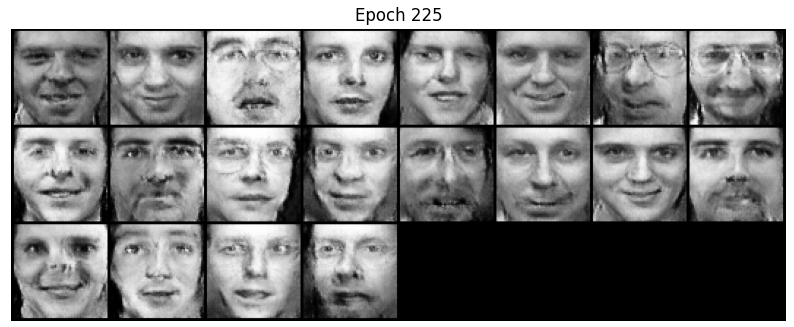
\includegraphics[width=0.45\textwidth]{/images_GAN_Olivetti_faces/epoch_225.png} \\
        Epoque 200 & Epoque 225 \\
        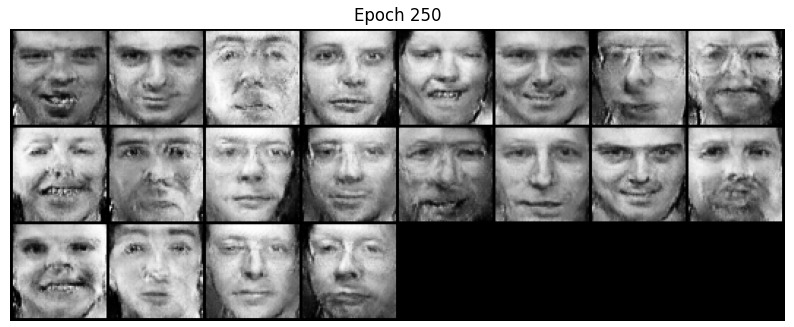
\includegraphics[width=0.45\textwidth]{/images_GAN_Olivetti_faces/epoch_250.png} &
        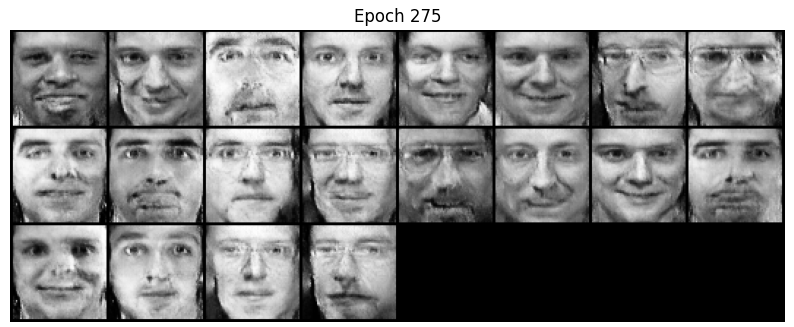
\includegraphics[width=0.45\textwidth]{/images_GAN_Olivetti_faces/epoch_275.png} \\
        Epoque 250 & Epoque 275 \\
        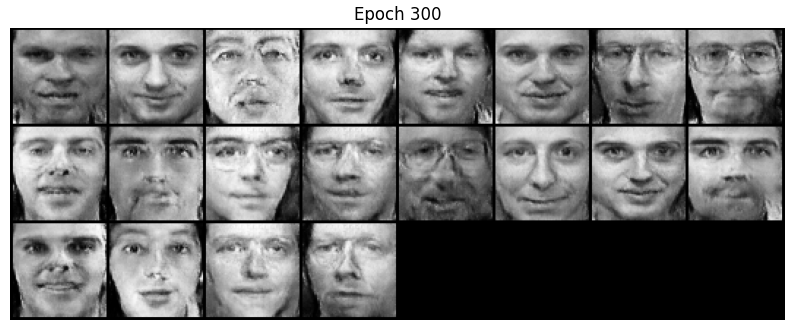
\includegraphics[width=0.45\textwidth]{/images_GAN_Olivetti_faces/epoch_300.png} & \\
        Epoque 300 & \\
    \end{tabular}
    \caption{Évolution du générateur sur le jeu de données Olivetti Faces}
\end{figure}
Le code permettant de générer de telles images se trouve \href{/gan_on_olivetti_faces.py}{ici}. \\
Google Colab a été utilisé pour générer ces images à l'aide d'un GPU T4 mais le programme fonctionne également sur
un simple CPU (le temps d'attente sera juste plus long).

\subsection{Etude de la génération de nouvelles images par le GAN}
Une question légitime à se poser est la suivante: un GAN génère t-il réellement de nouvelles images ou se contente-t-il
de copier des images du jeu d'entraînement ?
Pour répondre à cette question, on va étudier des GAN construit avec la même approche que ci-dessus. En revanche, on
utilise des images de visages pour plus facilement être capable de juger le lien entre les images. On n'entraîne les
réseaux qu'avec très peu de données:
Dans le cas à 3 images, on peut également voir apparaître une fusion des visages:
\begin{figure}[H]
    \centering
    \begin{tabular}{cc}
        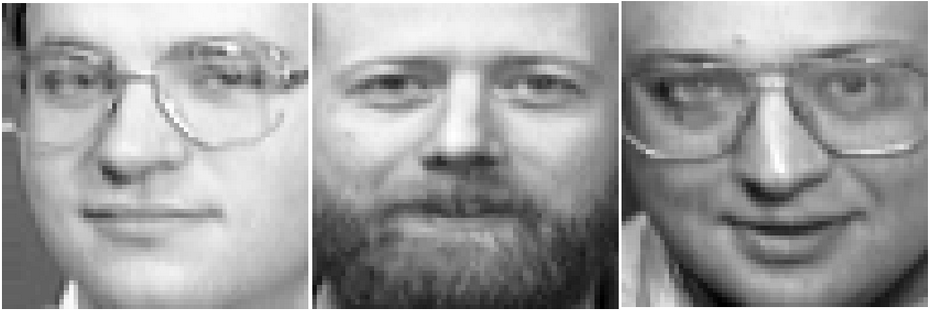
\includegraphics[width=0.45\textwidth]{/travail_session3/3_images_donnees.png} &
        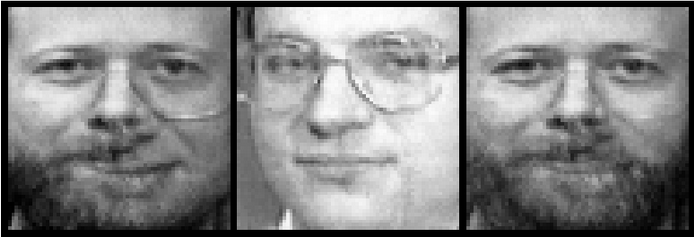
\includegraphics[width=0.45\textwidth]{/travail_session3/3_images_generees.png} \\
        Images issues de la BDD & Images générées par le GAN \\
    \end{tabular}
\end{figure}
Mais cette fusion des visages est en fait déjà visible à partir de 2 images:
\begin{figure}[H]
    \centering
    \begin{tabular}{cc}
        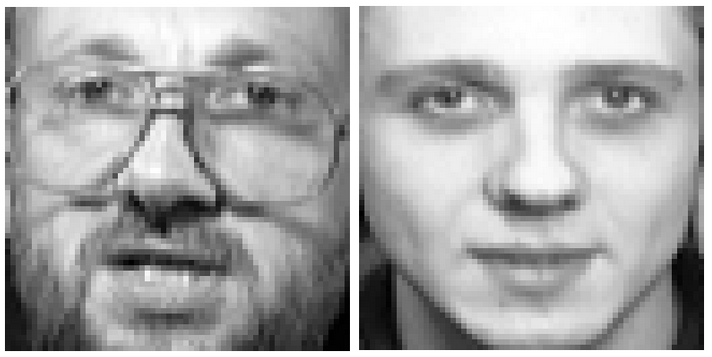
\includegraphics[width=0.45\textwidth]{/travail_session3/2_images_donnees.png} &
        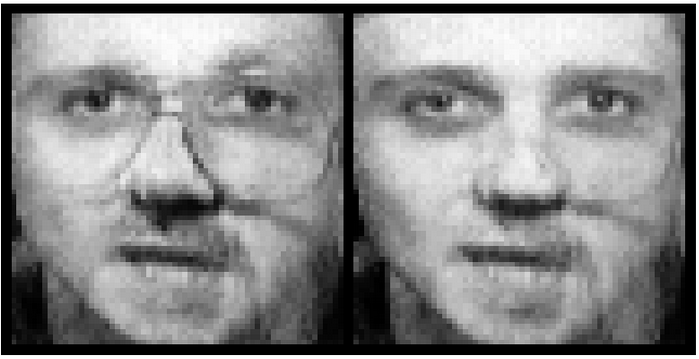
\includegraphics[width=0.45\textwidth]{/travail_session3/2_images_generees.png} \\
        Images issues de la BDD & Images générées par le GAN \\
    \end{tabular}
\end{figure}
Ce sont principalement les lunettes et la pilosité qui ont tendance à facilement se transmettre d'un visage à
l'autre. Il semble donc que les GAN aient réussi à discerner certains attributs.
En réalité, il est rare que le GAN produise constamment la même image puisqu'une telle situation engendrerait
forcément une \textit{loss} plus élevée et serait une situation instable.

Pour reproduire le code il suffit d'utiliser le code \href{/gan_on_olivetti_faces.py}{ici}, en réduisant la taille du dataset et en augmentant le nombre d'époques.

\subsection{Etude d'un GAN à 2 paramètres}
Jusqu'à présent, on n'a pas mis les mains dans les formules mathématiques, on a seulement utilisé des modules
python qui nous donnent une solution clé en main.
Pour plonger dans les calculs mathématiques derrière un GAN, on va s'attaquer à une version très simplifiée mais
sans utiliser de bibliothèque de machine learning. Notre problème simplifié consiste à générer des données en 2D selon
une \textit{gaussienne cible} de centre $(0,0)$. Pour cela le générateur construit des données selon une gaussienne
de même écart-type mais de centre $(x_{gen}, y_{gen})$ et on utilise un discriminateur sous la forme d'une fonction: 
$D(x,y) = e^{ -\frac{1}{2}((x-x_{dis})^2 + (y-y_{dis})^2) }$. \\
Les vraies données sont: $(X, Y) \sim N(x^*, y^*, \sigma)$. \\
Les données générées sont: $(Z, T) \sim N(x_{gen}, y_{gen}, \sigma)$. \\
On obtient deux fonctions de perte; la première que l'on doit maximiser, et la seconde que l'on doit minimiser: \\
$L_1 = \log(D(X,Y)) - \log(D(Z,T))$ \\
$L_2 = -\log(D(Z,T))$ \\
(On utilise les fonctions de pertes en log pour que l'exponentielle se simplifie). \\
Maintenant il nous faut étudier $ \theta = \begin{pmatrix}
x_d \\
y_d \\
x_g \\
y_g
\end{pmatrix} $.

\subsubsection{Sans partie aléatoire}
Dans un premier temps on suppose que les variables aléatoires ne sont pas aléatoires pour simplifier les calculs.
$$ \frac{\partial L_1}{\partial x_d} = (X - Z) $$
$$ \frac{\partial L_1}{\partial y_d} = (Y - T) $$
$$ \frac{\partial L_2}{\partial x_g} = (x_d - x_g) $$
$$ \frac{\partial L_2}{\partial y_g} = (y_d - y_g) $$
D'où l'équation différentielle suivante:
$$ \dot{\theta} = \alpha \times \begin{pmatrix}
0 & 0 & -1 & 0 \\
0 & 0 & 0 & -1 \\
1 & 0 & -1 & 0 \\
0 & 1 & 0 & -1
\end{pmatrix} \times \theta + \alpha \begin{pmatrix}
x^* \\
y^* \\
0 \\
0
\end{pmatrix} $$
Notons: $ M = \begin{pmatrix}
0 & 0 & -1 & 0 \\
0 & 0 & 0 & -1 \\
1 & 0 & -1 & 0 \\
0 & 1 & 0 & -1
\end{pmatrix} $. \\
$Sp(M) = \{ - \frac{1}{2} \pm i \frac{\sqrt{3}}{2} \}$. \\
$M$ peut donc être décomposée en une partie antisymétrique rotationnelle et une partie symétrique dissipative.
C'est pour cela que l'on peut obtenir des spirales lors de simulations.

\subsubsection{Avec partie aléatoire}
Maintenant on suppose que les variables sont aléatoires. On obtient toujours les mêmes dérivées partielles.
$$ \frac{\partial L_1}{\partial x_d} = (X - Z) $$
$$ \frac{\partial L_1}{\partial y_d} = (Y - T) $$
$$ \frac{\partial L_2}{\partial x_g} = (x_d - x_g) $$
$$ \frac{\partial L_2}{\partial y_g} = (y_d - y_g) $$ 
Mais l'équation différentielle contient un terme supplémentaire. Les $\epsilon_i$ sont des variables aléatoires indépendantes
qui suivent une \textit{gaussienne} cible de centre 0 et d'écart type $\sigma$.
$$ \dot{\theta} = \alpha \times \begin{pmatrix}
0 & 0 & -1 & 0 \\
0 & 0 & 0 & -1 \\
1 & 0 & -1 & 0 \\
0 & 1 & 0 & -1
\end{pmatrix} \times \theta + \alpha \begin{pmatrix}
x^* \\
y^* \\
0 \\
0
\end{pmatrix} + \alpha \begin{pmatrix}
\epsilon_1 \\
\epsilon_2 \\
2 \times \epsilon_3 \\
\epsilon_4
\end{pmatrix} $$

\end{document}